

\input{../Latex_Templates/Preamble_Presentation}


%%%%% TITLE PAGE

% \subject{}
\title{Stagnation points of harmonic vector fields and the domain topology}
\subtitle{Some applications of Morse theory}
%\subtitle{Blatt 0}
\author{Theo Koppenhöfer}
\date{\today}

\addbibresource{bibliography.bib}
\graphicspath{{../Art/}}
\graphicspath{{../Plots/}}
\graphicspath{{../Figures/}}

\tikzexternaldisable


\usepackage{transparent}

\newcommand{\openX}{\interior\brk*{X}}


\begin{document}

% \frame[plain]

% Frame 2
{
  \usebackgroundtemplate{%
  {\transparent{0.3}\includegraphics[trim=2cm 5cm 0 1cm,width=\paperwidth,height=\paperheight]{../Art/mainExample_005_edited.pdf}}}
\frame[plain]{\titlepage}
}

% Frame 3
% \frame[plain]{\tableofcontents }

\begin{frame}
  \begin{definition}[Harmonic vector field]
    Let $X\subset\R^d$ be a suitable domain.
    A function $f\colon X\to\R$ is \emph{harmonic} if it satisfies the equation
    \begin{align*}
      0=\Delta f=\sum_j\partial_j^2f\,.
    \end{align*}
    A vector field $u\colon X\to\R^d$ is \emph{harmonic} if it is locally the gradient of a harmonic function, that is locally $u=\nabla f$.
  \end{definition}
\end{frame}

\section{Introduction}
% {
%   \usebackgroundtemplate{%
%   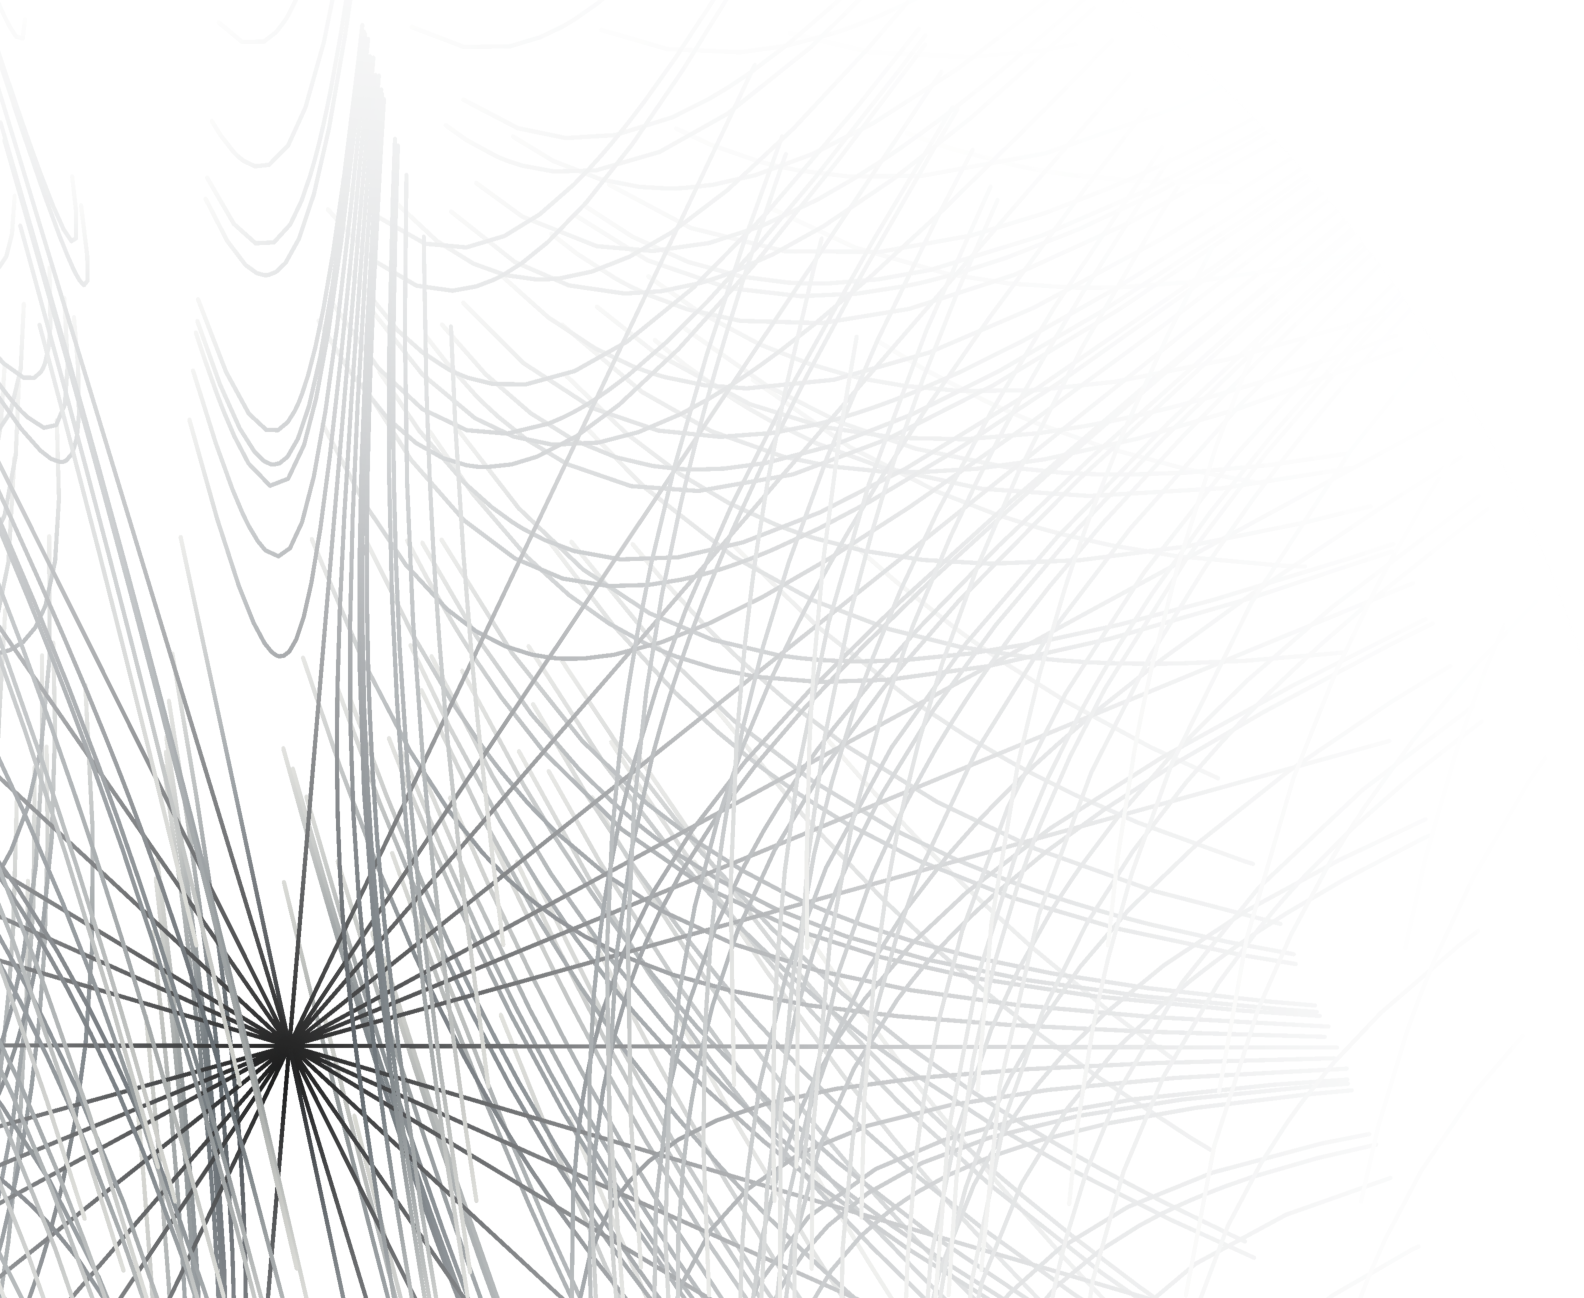
\includegraphics[trim=2cm 0 -30cm -30cm,width=\paperwidth,height=\paperheight]{../Art/centering_003_edited.pdf}}
\begin{frame}[fragile]
  \begin{block}{Why harmonic vector fields?}
    \begin{itemize}
      \item gravitational field in classical mechanics
      \item steady state heat flow
      \item irrotational flow of an inviscid incompressible medium
      \item electrostatic field in vacuum
      \item magnetostatic field in vacuum
    \end{itemize}
  \end{block}
\end{frame}
% }

\begin{frame}[fragile]
  \begin{definition}[Stagnation point]
    We call the zeros of a vector field $u\colon X\to\R^d$ \emph{stagnation points}.
  \end{definition}
  \begin{block}{Why stagnation points?}
    \tikzset{external/export=false}
    \[\begin{tikzcd}[column sep=huge]
      \text{vector field topology} \arrow[r,leftrightarrow,"\text{Morse theory}"] &\text{stagnation points}
    \end{tikzcd}\]
  \end{block}
  
\end{frame}

\section{Flowthrough with stagnation point}

\begin{frame}
  The following question is inspired by \cite{Alber1992}:
  \begin{question}[Flowthrough with stagnation point] \label{qu:flowthroughStagnationPoint}
    Does there exist a domain $X\subset\R^d$ homeomorphic to a ball and a harmonic vector field $u\colon X\to\R^d$ such that
    \begin{enumerate}
      \item $u$ has an interior stagnation point
      \item the boundaries on which $u$ enters and leaves the region are connected?
    \end{enumerate}
  \end{question}
\end{frame}

\begin{frame}
  \begin{proposition}[Negative answer to this question in $d=2$ dimensions]\label{pr:n2_negativeResult}
    Let $X\subset\R^2$ be a simply connected planar compact manifold with corners and let $f\colon X\to\R$ be harmonic, non-degenerate on the interior
    $\interior\brk*{X}$ and without irregular critical points.
    Let $\Sigma=\Sigma_{\leq0}\sqcup\Sigma_{\geq0}$ be a disjoint decomposition of the boundary into simply connected nonempty sets such that
    we have for the strictly entrant boundary $\Sigma^-\subseteq\Sigma_{\leq0}$ and for the strictly emergent boundary $\Sigma^+\subseteq\Sigma_{\geq0}$.
    Then $f$ has no interior critical point.
  \end{proposition}
\end{frame}

\begin{frame}
  \begin{proposition}[Negative answer for cylinders, {\cite{Wahlen2023}}]\label{pr:n3_inflowOutflowCylinder}
    Let $X=[0,1]\times \overline{U}\subset\R^d$ be a cylinder where $U\subset\R^{d-1}$ is a bounded open set with $C^1$ boundary.
    Let further $f\colon X\to\R$ be non-constant and
    harmonic such that the sides
    $[0,1]\times \partial U=\Sigma^0$ are the tangential boundary,
    the lid $\brk[c]{0}\times U=\Sigma^{\leq0}$ is the entrant boundary and
    the lid $\brk[c]{1}\times U=\Sigma^{\geq0}$ is the emergent boundary. 
    Then $f$ cannot have an interior critical point.
  \end{proposition}
  \begin{proof}
    See blackboard or \cite{Koppenhoefer2024}.
  \end{proof}
  
\end{frame}

\begin{frame}
  \begin{figure}
    \centering
    \input{../Figures/n3_cylinder.pdf_tex}
    \caption{This kind of situation is not possible.}
    \label{fi:n3_cylinder}
  \end{figure}
\end{frame}

\begin{frame}
  \begin{example}[Connected entrant boundary in $d=4$ dimensions]\label{ex:n4}
    Consider as domain $X=B_1\subset\R^4$ the unit ball and
    the harmonic function 
    \begin{equation*}
      \begin{aligned}
      f\colon X&\to \R \\
      x &\mapsto x_1^2+x_2^2-x_3^2-x_4^2\,.
      \end{aligned}
      \label{eq:n4_deff}
    \end{equation*}
    This has a critical point at the origin.
    It is shown in \cite{Koppenhoefer2024} that the entrant and emergent boundaries are in fact connected.
  \end{example} 
\end{frame}


\begin{frame}
  \begin{question}[Flowthrough with stagnation point] \label{qu:flowthroughStagnationPoint}
    Does there exist a domain $X\subset\R^d$ homeomorphic to a ball and a harmonic vector field $u\colon X\to\R^d$ on $X$ such that
    \begin{enumerate}
      \item $u$ has an interior stagnation point
      \item the boundaries on which $u$ enters and leaves the region are simply connected?
    \end{enumerate}
  \end{question}
  \begin{answer}
  \begin{itemize}
    \item $d=2$ dimensions: Not possible (known).
    \item cylinders in $d=3$ dimensions: Not possible (known).
    \item $d=3$ dimensions: Number of stagnation points has to be even.
    \item $d=4$ dimensions: Possible for $X=B_1$, $u=\nabla f$ with $$f=x_1^2+x_2^2-x_3^2-x_4^2\,.$$
  \end{itemize}
\end{answer}
\end{frame}

\begin{frame}
  But if one allows for holes in $d=2$ dimensions it becomes possible.
  \begin{figure}
    \centering
    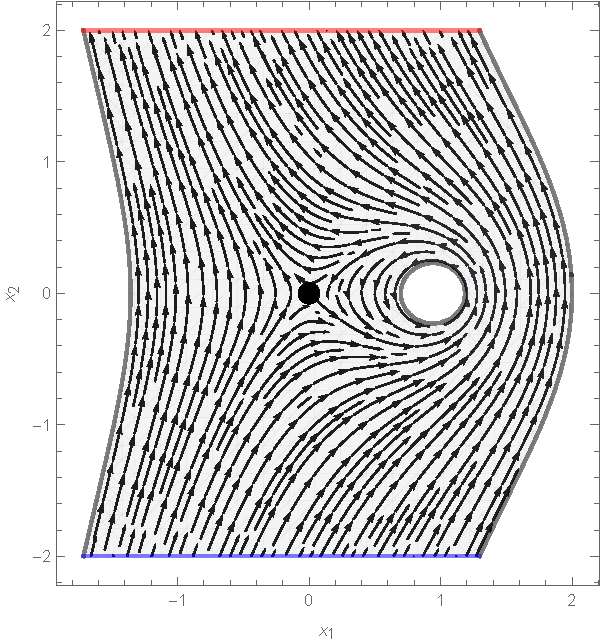
\includegraphics[width=0.5\textwidth]{../Plots/n2_hvf_InflowOutflow_asymmetric_gray_2.pdf}
    % 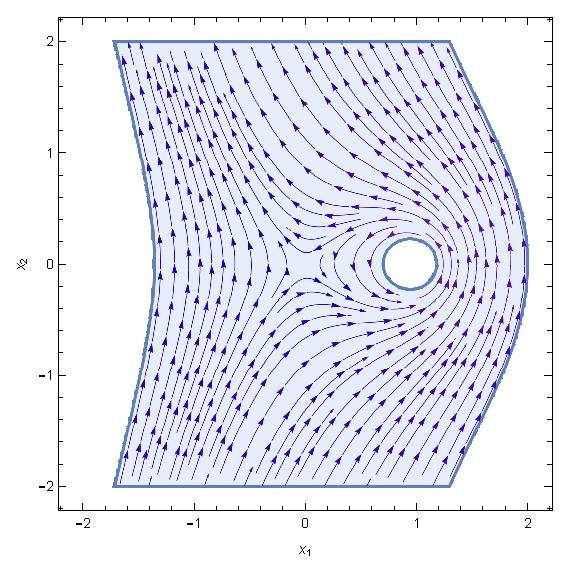
\includegraphics[width=0.6\textwidth]{../Plots/HarmonicVectorFields_gr3.eps}
    \caption{A plot of $u=\nabla^\perp\psi$ in the region $\psi^{-1}\brk*{[-0.5,2]}\cap \brk*{\R\times[-2,2]}$.
    Here $\psi\leftdef\Phi_2\brk*{x-e_1}+x_1$.}
    \label{pl:n2_hvf_InflowOutflow_asymmetric_single}
  \end{figure}
\end{frame}

\begin{frame}
  \begin{example}[A harmonic function with interior critical points and connected entrant and emergent boundaries]
    For $d=3$ dimensions we have for $r$ sufficiently large the example $X=B_r$, $u=\nabla f$ with
    \begin{align*}
      f=\frac{x_1^2}{2}-\frac{x_1^3}{3}-\frac{x_1x_2^2}{2}+x_1x_2^2+x_2x_3
    \end{align*}
  \end{example}
\end{frame}

\begin{frame}
  \begin{figure}
    \centering
    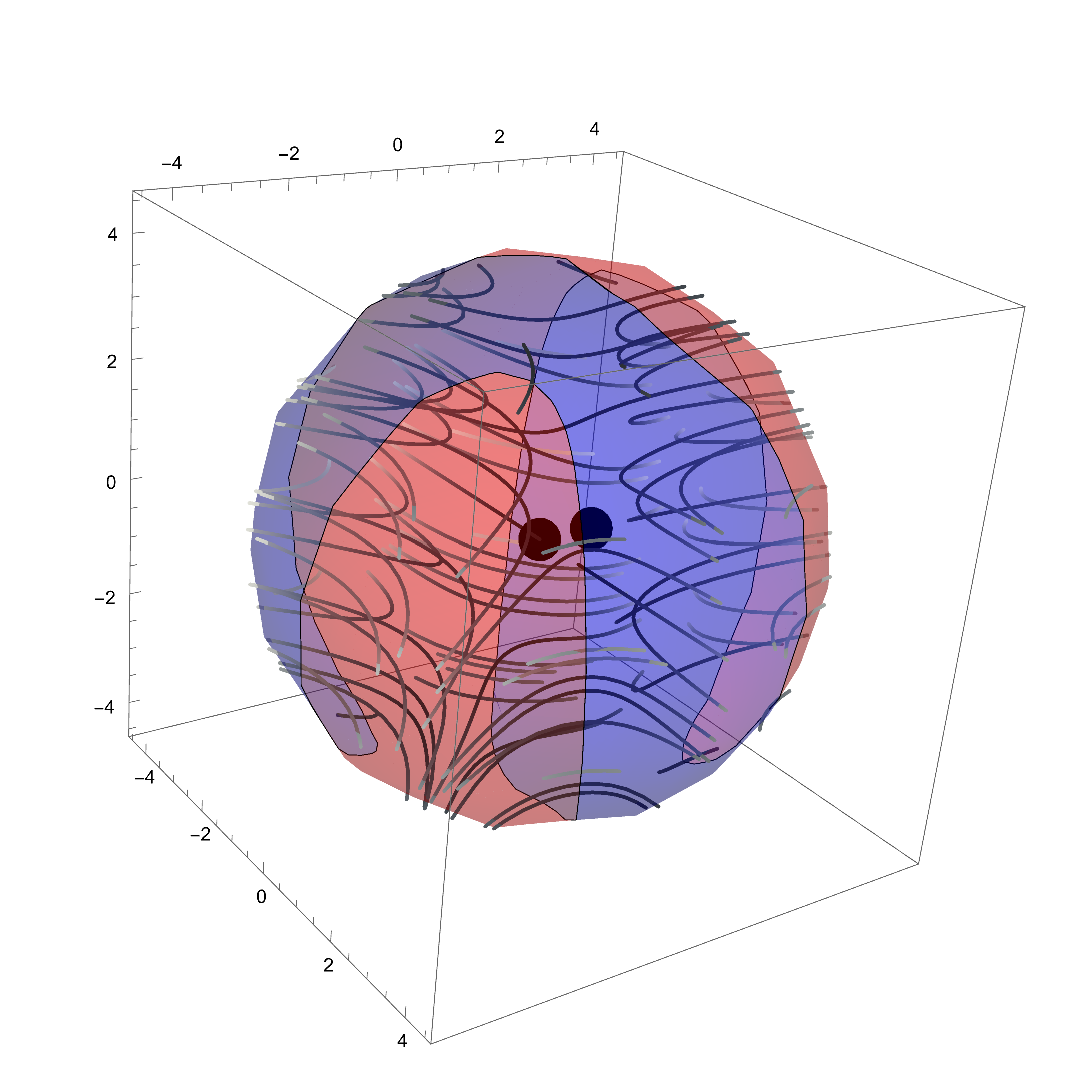
\includegraphics[width=0.6\textwidth]{../plots/n3_hf_inflowOutflow_Ball_overview.pdf}
    \caption{A stream plot of the function $u$. The interior stagnation points are highlighted in black.
    $\Sigma^+$ is shaded red, $\Sigma^-$ blue.}
    \label{pl:n3_hf_inflowOutflowStagnationPoint_overview}
  \end{figure}
\end{frame}

\begin{frame}
  \begin{figure}
    \centering
    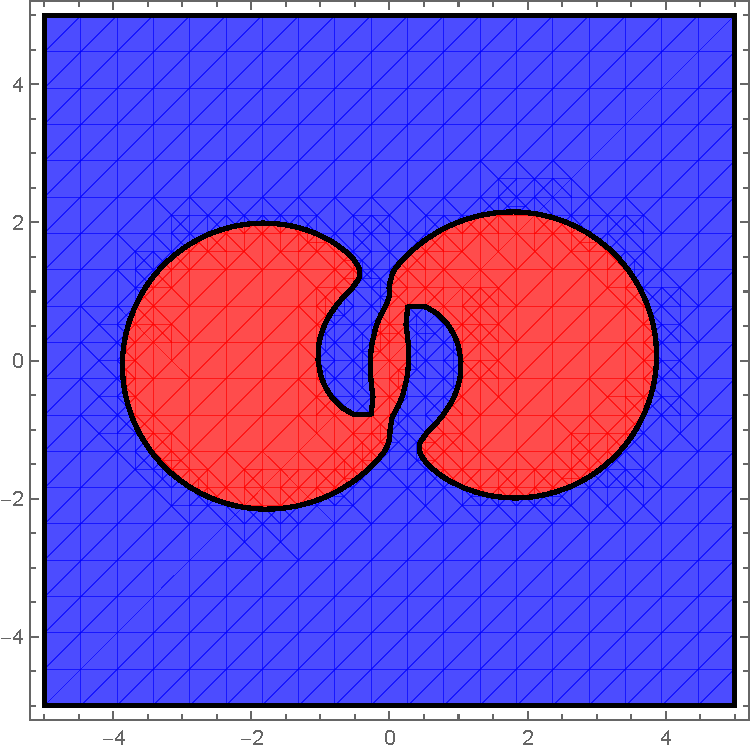
\includegraphics[width=0.6\textwidth]{../plots/n3_hf_inflowOutflow_Ball_Surface_2.pdf}
    \caption{Stereographic projection of the surface $\Sigma$. $\Sigma^+$ is shaded red, $\Sigma^-$ blue.}
    \label{pl:n3_hf_inflowOutflowStagnationPoint_Surface}
  \end{figure}
\end{frame}

\begin{frame}
  One can perturb this solution to show that there exists a harmonic vector field
  on $B_r$ with interior stagnation point such that $\Sigma^+$ and $\Sigma^-$ have positive distance
  from one another and are simply connected.
\end{frame}

\section{Harmonic vector fields without inflow or outflow}

\begin{frame}
  The following question is inspired by \cite{Lortz1970}:
  \begin{question}[Harmonic vector fields without inflow or outflow]
    Let $u$ be a harmonic vector field in a domain $X$ such that at every boundary point it is tangential to the boundary
    and non-vanishing.
    What can be said about the relation between the number of stagnation points and the domain topology?
  \end{question}
\end{frame}

\begin{frame}
  \begin{definition}[Interior stagnation points]
    Let $X\subset\R^d$ be a $d$-dimensional compact manifold with corners and $u\colon X\to\R^d$ be a vector field without boundary stagnation points.
    We call an interior stagnation point $x$ \emph{non-degenerate} if the derivative $Du(x)$ is bijective.
    If all interior stagnation points are non-degenerate $u$ is called \emph{Morse}.
  \end{definition}
\end{frame}

\begin{frame}
  % In $d=2$ dimensions one essentially has the relation
  % \begin{align*}
  %   M=\chi\brk*{X}
  % \end{align*}
  % where $M$ is the number of stagnation points and $\chi\brk*{X}$ the Euler characteristic of $X$.
  The following answers the question in $d=2$ dimensions:
  \begin{proposition}[Condition on the number of stagnation points, \cite{Koppenhoefer2024}]\label{pr:n2_hvf_noInflowNoOutflow}
    Let $X\subset\R^2$ be a compact connected planar manifold with corners
    and let $u\colon X\to\R^2$ be
    a Morse harmonic vector field without boundary stagnation points.
    Then we have the relation $M=-\chi(X)$ where $M$ denotes the number of stagnation points and
    $\chi(X)$ is the Euler characteristic of $X$.
  \end{proposition}
\end{frame}

\begin{frame}
  \begin{figure}
    \centering
    % 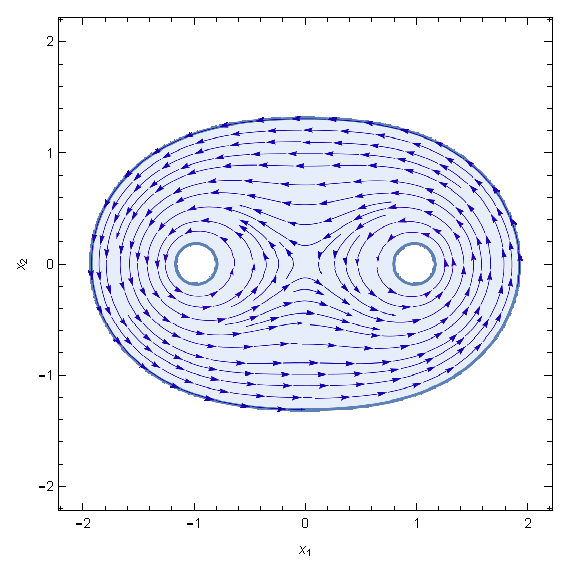
\includegraphics[width=0.6\textwidth]{../Plots/HarmonicVectorFields_gr1.eps}
    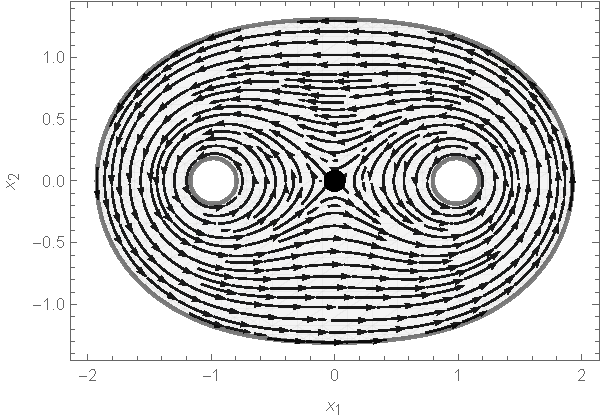
\includegraphics[width=0.9\textwidth]{../Plots/n2_hvf_noInflowNoOutflow_symmetric_gray_2.pdf}
    \caption{A plot of $u=\nabla^\perp\psi$ in the domain $\psi^{-1}\brk*{[-1,1]}$.
      Here $\psi\leftdef\Phi_2\brk*{x-e_1}+\Phi_2\brk*{x+e_1}$.}
    \label{pl:n2_hvf_noInflowNoOutflow}
  \end{figure}
\end{frame}

\begin{frame}
  \begin{example}[Stagnation points on the boundary]
    Let $X=\overline{B}_4\setminus\brk*{B_1\brk*{2e_1}\cup B_1\brk*{-2e_1}}$ be the domain and let the stream function $\psi$ be given by
    \begin{equation*}
      \begin{aligned}
        \Delta \psi&=0 &&\text{on }\openX, \\
        \psi&=0 &&\text{on the outer ring }4S^1, \\
        \psi&=-1 &&\text{on the left inner ring }S^1(-2e_1), \\
        \psi&=1 &&\text{on the right inner ring }S^1(2e_1),
      \end{aligned}\label{eq:n2:hvf:roundRegion:InflowOutflow}
    \end{equation*} 
  \end{example}
  
\end{frame}

\begin{frame}
  \begin{figure}
    \centering
    % 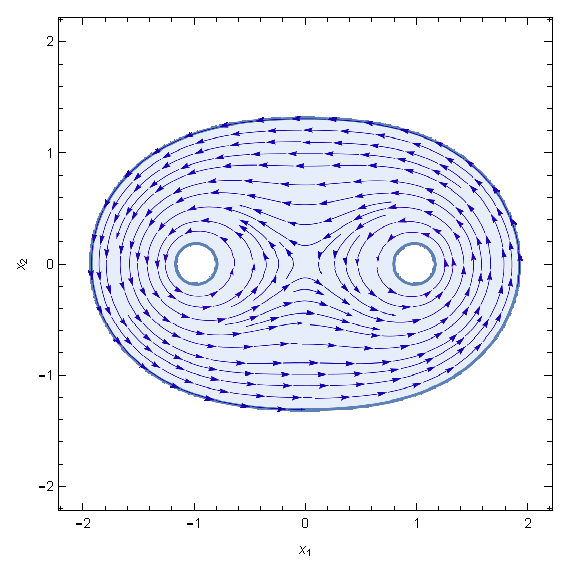
\includegraphics[width=0.6\textwidth]{../Plots/HarmonicVectorFields_gr1.eps}
    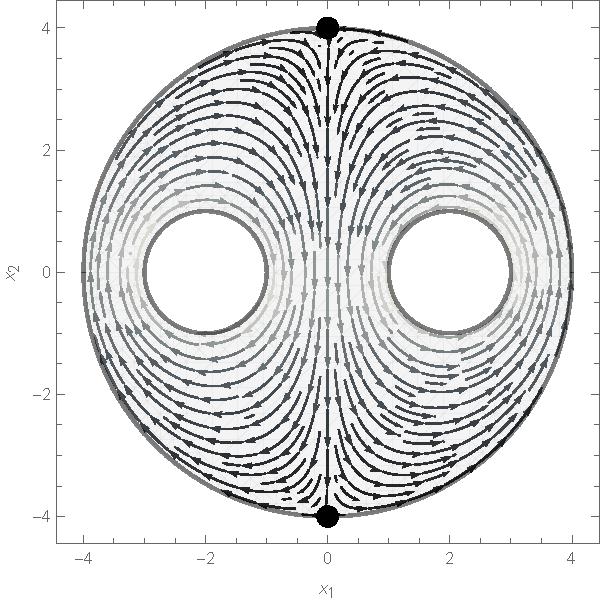
\includegraphics[width=0.6\textwidth]{../Plots/n2_hvf_roundRegion_InflowOutflow_gray_2.pdf}
    \caption{A plot of $u=\nabla^\perp\psi$ in the domain $X$ given as in the previous slide.}
    \label{pl:n2_hvf_noInflowNoOutflow}
  \end{figure}
\end{frame}

\begin{frame}
  \begin{definition}[Interior type number]
    Let $u\colon X\to\R^d$ be a Morse vector field without boundary stagnation points.
    We say that a stagnation point $x$ of $u$ has \emph{index $k$} if $Du$ has exactly $k$ negative eigenvalues.
    The \emph{interior type number} $M_k$ denotes the number of interior stagnation points of index $k$.
  \end{definition}
\end{frame}

\begin{frame}
  \begin{proposition}[Condition on the domain topology, \cite{Koppenhoefer2024}]\label{pr:n3_domainCond}
    Let $X$ be a compact orientable odd dimensional manifold with smooth boundary.
    Let further $u\colon X\to TX$ a smooth vector field with isolated stagnation points on the interior and without
    boundary stagnation points. Then the Euler characteristic of the domain $\chi\brk*{X}=0$ has to vanish.
  \end{proposition} 
\end{frame}

\begin{frame}
  \begin{corollary}[Condition on the type numbers and domain, \cite{Koppenhoefer2024}]\label{co:n3_conditionTypeNbrII}
    Let $X\subset\R^3$ be a compact three-dimensional manifold with smooth boundary and let further
    $u\colon X\to TX$ be a Morse harmonic vector field with no
    inflow or outflow through the boundary. Then
    we have the condition $M_1=M_2$ between the type numbers and the Euler characteristic of the domain $\chi\brk*{X}=0$ vanishes.
  \end{corollary}
\end{frame}



\section{Sources}

\begin{frame}[allowframebreaks]
	\frametitle{Sources}
	\nocite{*}

	% \bibliographystyle{plain}
	\setbeamertemplate{bibliography item}[text]
	% \bibliography{bibliographyFile}
	\printbibliography
\end{frame}

{
  \usebackgroundtemplate{%
  {\transparent{0.25}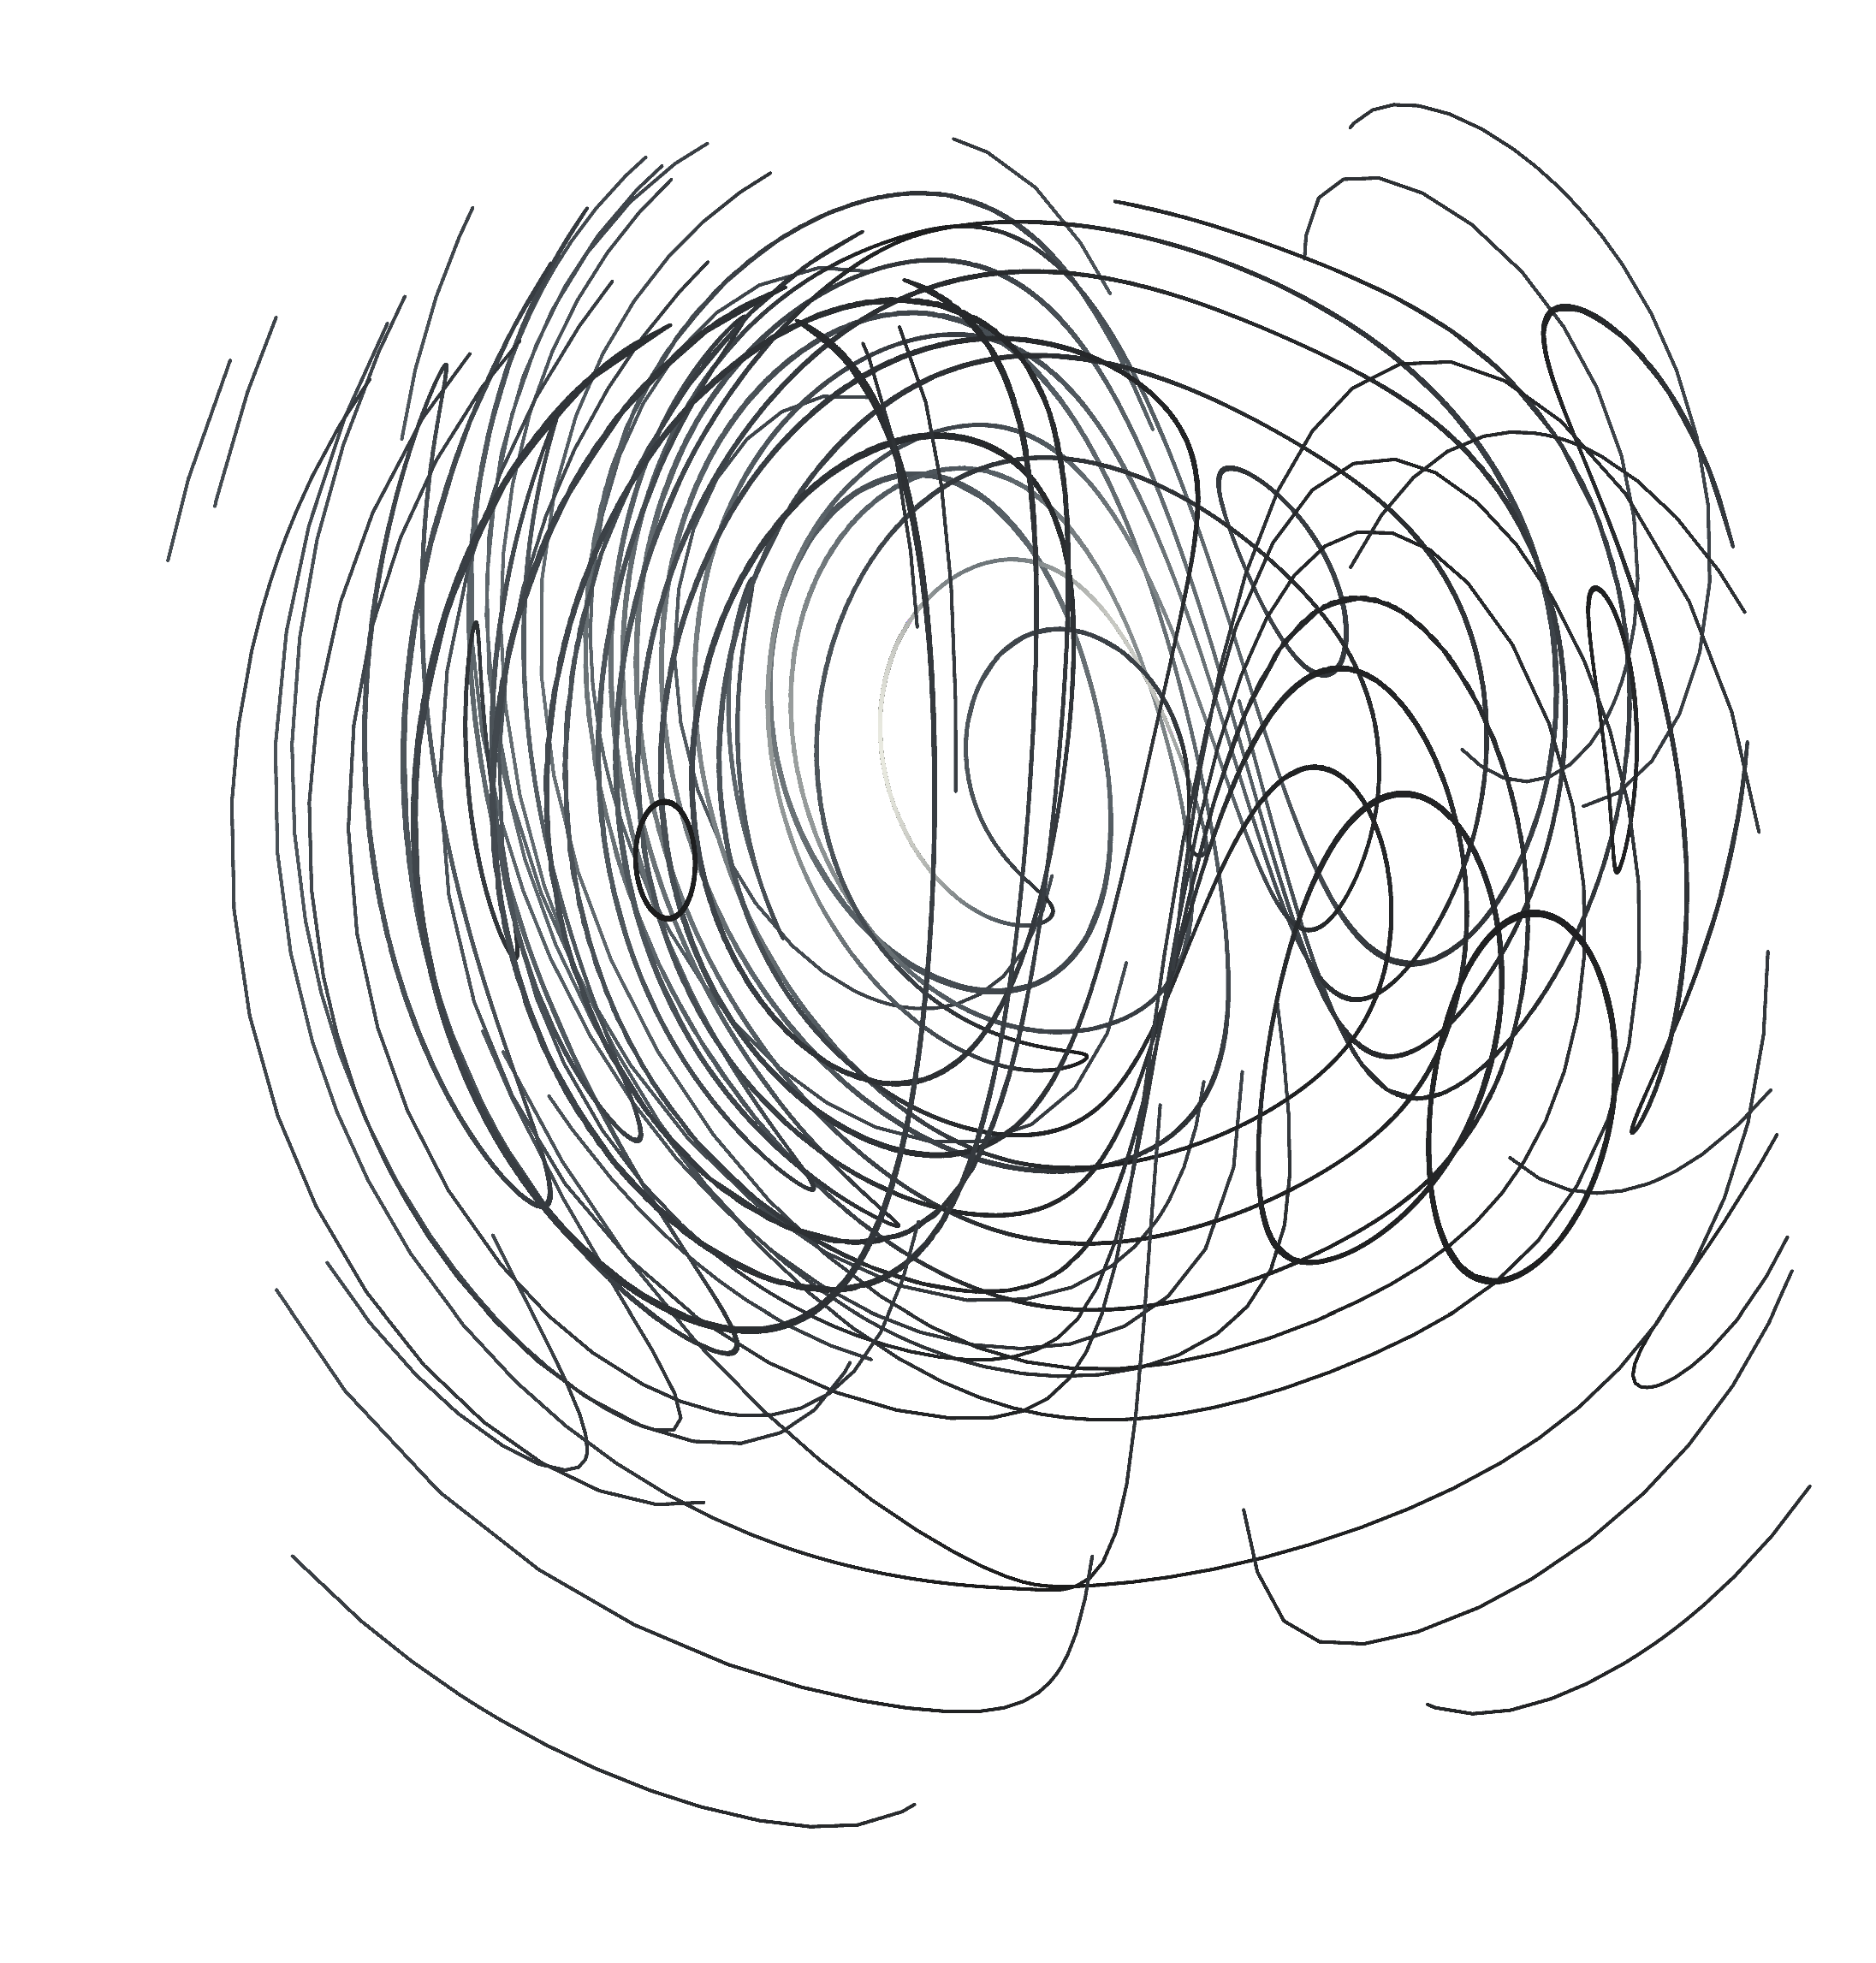
\includegraphics[trim=5cm 3cm 3cm 5cm,width=\paperwidth,height=\paperheight]{../Art/circular_001.pdf}}}
\begin{frame}[plain]
	\begin{center}
		\Large{{Thank you for your attention.}}
	\end{center}
\end{frame}
}

% \frame[plain]

\end{document}
